\documentclass[aspectratio=169,11pt]{beamer}
\usefonttheme{professionalfonts}
\renewcommand{\normalsize}{\fontsize{12}{15}\selectfont}
\usepackage[T1]{fontenc}
\usepackage{lmodern,amsmath,booktabs,tabularx,array,tikz}
\usetikzlibrary{arrows.meta,positioning}
\definecolor{navy}{HTML}{1D3550}
\definecolor{teal}{HTML}{147D83}
\definecolor{grey}{HTML}{596572}
\definecolor{rulegrey}{HTML}{D8DFE5}
\setbeamercolor{normal text}{fg=navy,bg=white}
\setbeamercolor{structure}{fg=teal}
\setbeamercolor{frametitle}{fg=navy,bg=white}
\setbeamerfont{frametitle}{size=\large,series=\bfseries}
\setbeamertemplate{navigation symbols}{}
\setbeamertemplate{itemize items}[circle]
\setbeamersize{text margin left=9mm,text margin right=9mm}
\setbeamertemplate{frametitle}{%
 \vspace{3mm}\insertframetitle\par\vspace{2mm}%
 {\color{rulegrey}\hrule height .4pt}\vspace{1mm}}
\setbeamertemplate{footline}{%
 \hspace{9mm}\begin{beamercolorbox}[wd=.86\paperwidth,ht=3ex,dp=1.5ex]{normal text}%
 \color{grey}\scriptsize Saarthak Krishan\hfill DH 307\hspace{5mm}\insertframenumber
 \end{beamercolorbox}}
\addtobeamertemplate{itemize/enumerate body begin}{\setlength{\itemsep}{4mm}}{}
\newcommand{\process}[3]{%
 \begin{center}
 \begin{tikzpicture}[node distance=10mm,every node/.style={font=\small\bfseries},every path/.style={draw=teal,line width=.8pt}]
 \node (a) {#1}; \node[right=of a] (b) {#2}; \node[right=of b] (c) {#3};
 \draw[-{Latex}] (a)--(b); \draw[-{Latex}] (b)--(c);
 \end{tikzpicture}
 \end{center}\vspace{2mm}}
\newcommand{\conclusion}[1]{\par\vspace{4mm}\noindent{\color{teal}\bfseries #1\par}}
\title{Protein--Ligand Design}
\subtitle{Cooperative and Conformation-Aware Search}
\author{Saarthak Krishan}
\institute{Supervised by Prof. Debabrata Maiti}
\date{}

\begin{document}
\begin{frame}[plain]
 \vspace{7mm}
 {\color{grey}\small DH 307 Research Progress\par}
 \vspace{7mm}
 {\bfseries\fontsize{25}{30}\selectfont Protein--Ligand Design\par}
 \vspace{3mm}
 {\large Cooperative and Conformation-Aware Search\par}
 \vspace{4mm}
 {\color{teal}\rule{24mm}{1pt}\par}
 \vspace{3mm}{\small Exploratory study: methods, observations and next steps\par}
 \vspace{6mm}
 Saarthak Krishan\\[1mm]
 {\small Roll No. 22B3959}\\[3mm]
 {\small Supervised by Prof. Debabrata Maiti}
\end{frame}

\begin{frame}{Two generation directions, two search settings}
 \begin{columns}[T]
 \column{.47\textwidth}
 \textbf{Ligand generation}\par
 \[q_\theta(L\mid P)\]
 Generate ligand $L$ for pocket $P$.
 \column{.47\textwidth}
 \textbf{Pocket generation}\par
 \[q_\phi(P\mid L,S)\]
 Design a pocket for a ligand, within scaffold $S$.
 \end{columns}
 \vspace{5mm}
 \begin{itemize}
 \item \textbf{Cooperative:} coordinate ligand and permitted pocket changes.
 \item \textbf{Conformation-aware:} choose ligands across states of a fixed protein sequence.
 \end{itemize}
 \conclusion{Can learned selection improve the search in either setting?}
 {\small\color{grey}$q$: conditional generative distribution. The directions are many-to-many.}
\end{frame}

\begin{frame}{Setting 1: cooperative co-design}
 \process{Ligand choice}{Pocket choice}{Shared reward}
 \begin{enumerate}
 \item FLOWR proposes ligands; PocketGen proposes pocket edits.
 \item The policies select a ligand and a complementary pocket edit.
 \item Evaluate the pair; update both policies with the same reward.
 \end{enumerate}
 \vspace{3mm}
 \[r_L=r_P=U(P_{t+1},L_{t+1})-U(P_t,L_t)-c\]
 {\small $U$: pair utility; $c$: cost per decision. Infeasible moves receive a penalty.}
 \conclusion{Hypothesis: coordination improves on one-sided search.}
 {\small\color{grey}Backbone preserved; at most four mutations. Application: engineered pairs.}
\end{frame}

\begin{frame}{Setting 2: conformation-aware ligand search}
 \process{Ligand choice}{Difficult conformation}{Opposite rewards}
 \begin{enumerate}
 \item Build a local conformation ensemble with restrained molecular dynamics.
 \item The ligand policy selects a generated molecule.
 \item The opposing policy selects a difficult state of the same protein.
 \end{enumerate}
 \vspace{3mm}
 \[r_L=U(P_C,L),\qquad r_C=-U(P_C,L)\]
 {\small $P_C$: conformation selected by the opposing policy; protein sequence stays fixed.}
 \conclusion{Hypothesis: difficult states encourage more robust ligand choices.}
\end{frame}

\begin{frame}{Where the RL layer connects}
 \begin{center}
 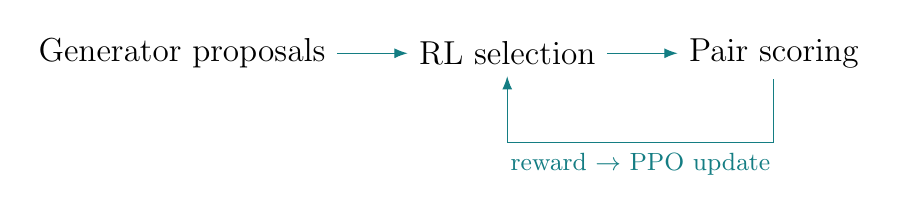
\begin{tikzpicture}[node distance=9mm,every node/.style={font=\normalsize}]
 \node (a) {Generator proposals};
 \node[right=of a] (b) {RL selection};
 \node[right=of b] (c) {Pair scoring};
 \draw[-{Latex},teal] (a)--(b);
 \draw[-{Latex},teal] (b)--(c);
 \draw[-{Latex},teal] (c.south)--++(0,-8mm)-| node[pos=.25,below,font=\small] {reward $\rightarrow$ PPO update} (b.south);
 \end{tikzpicture}
 \end{center}
 \vspace{3mm}
 \begin{itemize}
 \item \textbf{Observation:} molecular descriptors, pocket composition and contact geometry.
 \item \textbf{Action:} choose a ligand plus a pocket edit or protein conformation.
 \item \textbf{Learning:} PPO updates the selection policies; pretrained generators supply the proposals.
 \end{itemize}
 \conclusion{RL learns which proposals to select over repeated decisions.}
\end{frame}

\begin{frame}{How a protein--ligand pair is evaluated}
 \[\boxed{U(P,L)=-V(P,L)-0.01E(L)-0.05N(P)}\]
 \vspace{3mm}
 \begin{tabularx}{\textwidth}{@{}p{15mm}>{\raggedright\arraybackslash}X@{}}
 $V(P,L)$ & Vina score at the supplied ligand pose; more negative is better.\\[4mm]
 $E(L)$ & Ligand strain: MMFF94s energy before minus after minimization.\\[4mm]
 $N(P)$ & Number of mutated residues relative to the starting protein.\\
 \end{tabularx}\par
 \vspace{4mm}
 Chemical and geometric checks determine whether a pair is feasible.
 \conclusion{Higher utility is better; strain and mutations carry penalties.}
 {\small\color{grey}This is a computational proxy for compatibility.}
\end{frame}

\begin{frame}{Cooperative results: learning remains close to random search}
 \noindent{\small Three completed policy seeds. Higher utility is better.\par}
 \vspace{4mm}
 \begin{tabularx}{\textwidth}{@{}Xr@{}}
 \toprule
 Method & Mean utility\\
 \midrule
 Learned cooperative policy & \textbf{6.350}\\[2mm]
 Random joint search & 6.301\\[2mm]
 Greedy alternating & 6.227\\[2mm]
 Ligand-only & 5.902\\
 \bottomrule
 \end{tabularx}\par
 \vspace{4mm}
 {\small The paired uncertainty interval for learned minus random includes zero.\\[2mm]
 Ligand-only search often had no eligible new candidate.}
 \conclusion{These results do not yet establish a reliable RL advantage.}
\end{frame}

\begin{frame}{Current bottlenecks: imbalance and eligibility}
 \begin{columns}[T]
 \column{.47\textwidth}
 \textbf{Cooperative search}\par\vspace{3mm}
 \begin{itemize}
 \item Pocket edits are available more often than eligible ligand changes.
 \item Learned and random joint search perform similarly.
 \end{itemize}
 \column{.47\textwidth}
 \textbf{Competitive search}\par\vspace{3mm}
 \begin{itemize}
 \item De novo proposals face a reference-similarity restriction.
 \item Audited case: 64 generated, 62 valid, zero eligible for scoring.
 \end{itemize}
 \end{columns}
 \vspace{5mm}
 \textbf{Working hypothesis:} unequal proposal quality and availability limit learning.
 \conclusion{Measure the imbalance before changing the game or training schedule.}
\end{frame}

\begin{frame}{Next phase: distillation and balanced learning}
 \begin{enumerate}
 \item \textbf{Align proposals with the task.} Match generation to the eligibility criteria; handle empty action sets.
 \item \textbf{Distill a search teacher, then refine with PPO.} Use feasible high-utility search decisions to initialize the selection policies.
 \item \textbf{Balance and test both sides.} Measure proposal yield and reward influence; test extra updates for the weaker side.
 \end{enumerate}
 \conclusion{Compare imitation, PPO, and imitation + PPO under equal budgets.}
 {\small\color{grey}Distillation and balancing are proposed experiments.}
\end{frame}

\begin{frame}[plain]
 \vfill
 {\bfseries\fontsize{28}{34}\selectfont Thank you\par}
 \vspace{4mm}{\color{teal}\rule{24mm}{1pt}\par}
 \vspace{4mm}Saarthak Krishan
 \vfill
\end{frame}
\end{document}
